
\subsection{Jelek feldolgoz\'asa}

A jelfeldolgoz\'asra t\"obb matematikai m\'odszer is van, mind analitikus, mind numerikus t\'eren.
A vizsg\'alat t\'argy\'at most a diszkr\'et Fourier transzform\'aci\'o szolg\'alja.

\subsubsection{FFTW++}
Az \href{http://www.fftw.org/}{FFTW} egy szabad C k\"onyvt\'ar diszkr\'et Fourier transzform\'aci\'o sz\'am\'it\'as\'ara.
E k\"or\'e \'ep\'it kiss\'e bar\'ats\'agosabb \'es k\"onnyebben haszn\'alhat\'o k\"ornyezetet az \href{http://fftwpp.sourceforge.net/}{FFTW++}.
A javaslat az, hogy egy speci\'alis nagyteljes\'itm\'eny\H u \code{Array} oszt\'alyt haszn\'aljunk ezzel.

\"Osszehasonl\'it\'asra ker\"ult az a megold\'as is, ami nem haszn\'alja ezt az oszt\'alyt.

\subsubsection{Sz\'am\'it\'as GPU-n Vulkan-nal}
Ugyanakkor a Vulkan API sz\'am\'it\'asi feladatokat is el tud l\'atni nem csak grafikait. 
Mivel a grafikus visszajelz\'est c\'elszer\H u egy grafikai hardvereszk\"oz seg\'its\'eg\'evel v\'egezni adja mag\'at a lehet\H os\'eg, hogy helyben v\'egezz\"uk a sz\'am\'it\'ast, ezzel kor\'abban elv\'egezve az eszk\"oz saj\'at mem\'ori\'aj\'ara t\"ort\'en\H o m\'asol\'ast.

Mivel egy Vulkan sz\'am\'it\'asi h\'iv\'as aszinkron m\H uk\"odik, a fair \"osszehasonl\'it\'as \'erdek\'eben megv\'arja a m\'er\'es a feladat befejezt\'et. Azonban a p\'arhuzamos\'it\'as miatt, \'es mivel egyazon API haszn\'alat\'ar\'ol van sz\'o, ezt ki lehet haszn\'alni egy\'eb k\'es\H obbi optimaliz\'al\'asokra p\'eld\'aul a megjelen\'it\'es kapcs\'an.

\subsubsection{K\"ornyezet}
A tesztel\H o program megtal\'alhat\'o \href{https://github.com/petii/efop-signalproc}{GitHub-on}. 
A program param\'eterezhet\H o, hogy mekkora alap ablakm\'eret szorz\'okkal futtasson m\'er\'eseket, illetve egyes m\'er\'eseket h\'anyszor ism\'etelje meg. 
Ezeket az adatokat \code{.csv} f\'ajlokba export\'alja. Az adatokat egy egyszer\H u \code{R} szkript seg\'tis\'eg\'evel elemezhetj\"uk.

A teszt bemeneti adatok \href{https://en.cppreference.com/w/cpp/numeric/random/normal_distribution}{pszeudov\'eletlen sz\'amok a standard norm\'alis eloszl\'asb\'ol}.

\subsection{M\'er\'esek}
A k\'et f\H o m\H uvelet ami m\'er\'esre ker\"ult az adatok m\'asol\'asa illetve a DFT futtat\'asa.

\paragraph{Eszk\"oz\"ok}
\begin{itemize}
	\item Egy asztali g\'ep
	\begin{itemize}
		\item \href{https://ark.intel.com/products/80817/Intel-Core-i5-4460-Processor-6M-Cache-up-to-3_40-GHz}
		{Intel Core-i5 4460}
		\item \href{https://www.geforce.com/hardware/desktop-gpus/geforce-gtx-960}
		{NVIDIA GeForce GTX 960}
	\end{itemize}
	\item Egy laptop
	\begin{itemize}
		\item \href{https://ark.intel.com/products/76308/Intel-Core-i5-4300U-Processor-3M-Cache-up-to-2_90-GHz}
		{Intel Core-i5 4300U}
		\item Intel HD Graphics 4400
	\end{itemize}
\end{itemize}

\subsubsection{Eredm\'enyek}



\paragraph{M\'asol\'as}

\begin{figure}[h]
	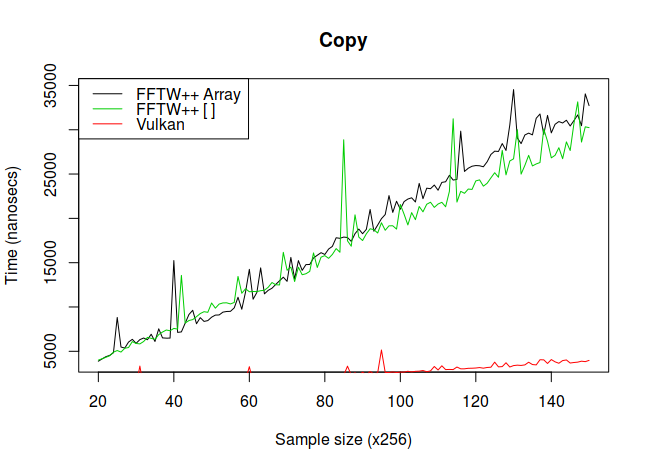
\includegraphics[width=\columnwidth]{copy-l-20-100-150}
	{4300U}
	%\includegraphics[width=\columnwidth]{}
	%{4460}
	\centering
	\caption{M\'asol\'as fut\'asi ideje}
\end{figure}

A m\'er\'esi eredm\'enyeket tartalmaz\'o \'abta $100$ futtat\'as eredm\'enyeinek \'atlag\'at mutatja.

A bemenet \'atm\'asol\'as\'ara ir\'anyul\'o m\'er\'esek olyan szempontb\'ol nem meglep\H oek, hogy nagyj\'ab\'ol line\'aris a bemenet m\'eret\'evel.

\paragraph{Transzform\'aci\'o}

\begin{figure}[h]
	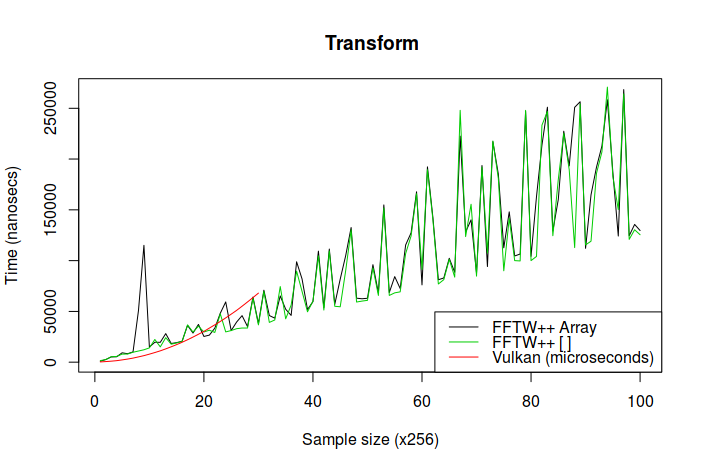
\includegraphics[width=\columnwidth]{transf-1-100}
	{4300U}
	%\includegraphics[width=\columnwidth]{}
	%{4460}
	\centering
	\caption{Transzform\'aci\'o fut\'asi ideje}
\end{figure}

